
\documentclass{IOS-Book-Article}

\usepackage{mathptmx}
\usepackage{soul}\setuldepth{article}
\usepackage{booktabs}
%\usepackage{times}
%\normalfont
%\usepackage[T1]{fontenc}
%\usepackage[mtplusscr,mtbold]{mathtime}
%
\usepackage{graphicx}
\usepackage{hyperref}
%\renewcommand\UrlFont{\color{blue}\rmfamily}
\setlength{\parskip}{0pt}
\raggedbottom
\usepackage{multirow}
\usepackage{amsmath}
\usepackage{csquotes}
\usepackage{paralist}
\usepackage{booktabs}
\usepackage{mathptmx}
\def\hb{\hbox to 10.7 cm{}}
\usepackage{pgfplots}
\pgfplotsset{compat=1.8}
\usepackage{subfigure}
\pgfplotsset{width=7cm,compat=1.8}
\usepackage{pgfplotstable}
%\renewcommand*{\familydefault}{\sfdefault}
\usepackage{tikz}

\def\hb{\hbox to 10.7 cm{}}

\begin{document}

\pagestyle{headings}
\def\thepage{}

\begin{frontmatter}              % The preamble begins here

%\pretitle{Pretitle}
\title{On the efficiency of Machine Learning Models in predicting Malaria using Sympt\^om Data}

\markboth{}{January 2020\hb}
%\subtitle{Subtitle}

\author{\fnms{Ousseynou} \snm{Mbaye}},
\author{\fnms{Mouhamadou Lamine} \snm{BA}
\thanks{Corresponding Author: Mouhamadou Lamine BA, LIMA, Universit\'e Alioune Diop,
BP.3400 Bambey, Senegal; E-mail: mouhamadoulamine.ba@uadb.edu.sn.}}
and
\author{\fnms{Alassane} \snm{SY}}

\runningauthor{O.Mbaye et al.}
\address{LIMA, Universit\'e Alioune Diop, Bambey, Senegal}
%\address[B]{Short Affiliation of Second Author and Third Author}

\begin{abstract}
Still today, Malaria remains one of the most feared diseases in Sub-Saharan Africa and especially in Senegal. This is mainly due to inappropriate medical care support coupled with an often late and error-prone diagnosis from the medical staff. In addition, largely used diagnostic standards such as the Rapid Diagnosis Test is not fully reliable. With the development and increasing adoption of automated tools in the health field, machine learning applications might help medical actors in their decision-making process. In this paper, we propose an experimental study of six machine learning algorithms for the prediction of Malaria in Senegal. These algorithms aim at predicting whether or not a given patient suffers from Malaria based on his signs and symptoms. The performance of the algorithms have been extensively tested and evaluated over real data sets about patients in Senegal that suffer or not from Malaria. The algorithms are evaluated using four criteria: accuracy, Recall, F-measure, Precision and Specificity. The research has shown that there is not necessarily a single best classification tool, but instead the best performing algorithm will depend on the dataset to be analysed.
\end{abstract}

\begin{keyword}
electronic camera-ready manuscript\sep IOS Press\sep
\LaTeX\sep book\sep layout
\end{keyword}
\end{frontmatter}
\markboth{January 2020\hb}{January 2020\hb}
%\thispagestyle{empty}
%\pagestyle{empty}

\section{Introduction}\label{Introduction}
Malaria is a life-threatening disease caused by parasites that are transmitted to people through the bites of infected female Anopheles mosquitoes. It is preventable and curable. Malaria is an acute febrile illness. In a non-immune individual, symptoms usually appear 10–15 days after the infective mosquito bite. The first symptoms – fever, headache, and chills – may be mild and difficult to recognize as malaria. If not treated within 24 hours, P. falciparum malaria can progress to severe illness, often leading to death. Children with severe malaria frequently develop one or more of the following symptoms: severe anaemia, respiratory distress in relation to metabolic acidosis, or cerebral malaria. In adults, multi-organ failure is also frequent. In malaria endemic areas, people may develop partial immunity, allowing asymptomatic infections to occur. In 2019, there were an estimated 229 million cases of malaria worldwide. The estimated number of malaria deaths stood at 409 000 in 2019. The WHO African Region carries a disproportionately high share of the global malaria burden. In 2019, the region was home to 94\% of malaria cases and deaths, thanks to the  2019 World Malaria Report \cite{19WMR}. 
Over the past years, many efforts have been done by governmental and non governmental organizations  to eradicate Malaria:  actions continuously conducted by the WHO are real examples of those.  In the research field, many studies, aiming at understanding the disease from the Plasmodium mosquito point of view or proposing automated detection tools, have been conducted \cite{Ga19,Le74,ermert2011development,Hu17}. The Rapid Diagnostic Test (RDT) \cite{Hu17} is one of the most successful and prominent introduced tool to automatically predict whether or not a given patient suffers from Malaria. It relies on the
detection of specific Plasmodium proteins, PfHRP2, pLDH
and aldolase. The RDT is largely used and adopted as a standard in many health structures in Sub-African countries because of its simplicity to utilize and does not require any specific domain knowledge. However as highlighted in \cite{Hu17} the RDT is not fully reliable:  in Section \ref{Methods} we show that the precision of the RDT is about 90\% for the real datasets used in this study.
With the development and increasing adoption of automated tools in the health field, machine learning  (ML) \cite{mitchell1997machine, Ug1} applications might help medical actors in their decision-making process. 
 In this paper, we propose an  extensive comparative study of six machine learning algorithms, among the most popular for the prediction of Maria in Senegal. The evaluated and compared ML algorithms are Naive Bayes (NB), Logistic Regression(LR) ,  Decision Tree(DT), Support Vector Machine(SVM) ,
 Random Forest(RF),
 and Artificial Neural Network(ANN). We conducted experiments on five datasets based on the two real world datasets about Senegalese citizens that suffer or not from Malaria. These two datasets have been collected in two different contexts and contain clinical data such as sign, symptom and final diagnostic of patients living in distinct locations in Senegal (for the first dataset) or within the same area (for the second dataset). Those patients have been examined by doctors in given health services and their clinical data recorded: for each patient the final diagnostic is provided with the corresponding signs and symptoms. The outcome of the RDT is also provided. 
% paper organization
The rest of the paper is structured as follows.First we gives detail explanation of machine learning metthods and the different data sets methods used for this study in section 2. In section 3 our  differents results are presented. Section 4 and 5 includes discussion of our results and conclusions of this paper.
 \newpage

% Prediction Model
\section{Methods}\label{Methods}
In this part we discusse about the methods and the technic of machine learning used in this study
\subsection{Methodology}

\subsection{Machine Learning algorithms}
In the following we discuss about some of these methods.  Those algorithms are chosen among the most used ones in the health field according to studies\cite{de2018binary,tomar2013survey}.\\
\textbf{Decision tree (DT)}\cite{Ro05} is a supervised classifier which is obtained by recursively partitioning the labelled set of observations. It is one of the most adopted classifiers, thanks to its simplicity and its straightforward interpretation. For CART algorithms, hyperparameters are the impurity criteria (entropy and gini), the maximum depth, the minimum samples to split and the minimum samples at a leaf

% Random forest
\textbf{Random Forest (RF)}\cite{Be01} is an ensemble approach built upon many decision tree classifiers. It is a supervised classifier which requires the same hyper parameters as DT, plus the number of trees to create and the random number of features to look at when splitting the labelled data during the training step \cite{Be01}.\\
% Naive Bayes
\textbf{ Naive Bayes classifier (NB) }\cite{Ka17} is a\emph{supervised} machine learning algorithm, i.e. requires to be trained, used for classifying observations to given distinct classes based on \emph{input explanatory variables} (a.k.a feature or attribute).
It is a classification technique based on the well-known \emph{Bayes’ theorem}\footnote{https://en.wikipedia.org/wiki/Bayes\%27\_theorem} with strong and naive assumptions. It simplifies learning by assuming that features are independent of given class.\\
% Logistic Regression 
\textbf{Logistic regression (LR)} \cite{Ph88} is a statistical model used in the machine learning domain as a supervised classifier for binary classification \cite{uddin2019comparing}. 
It is based, in its basic form, on a logistic function to describe a binary dependent variable\cite{wang2014support,de2018binary} by considering as input 
qualitative or/and ordinal explanatory variables  in order to measure the probability of a given class label. The greatest advantage  of the logistic regression
classifier is the fact that you can use continuous explanatory variables and it is easier to handle more than two explanatory variables simultaneously and its ability to quantify the strength of the relationship between each explicative variable and the variable to explain, given the other variables integrated to the model.\\
%Support Vector Machine
\textbf{Support Vector Machine (SVM)} \cite{Ev01} is a supervised classification approach whose intuition is to represent input data in a space and to determine the optimal hyper-plane that divides that space in two regions depending on the targeted value.\\
% artificial neural networks
\textbf{An Artificial Neural Network (ANN)} \cite{Me19} is a computational approach also referred to as a Connectionist System used in Machine Learning. ANNs are loosely modeled after the biological neural network in an attempt to replicate the way in which we learn as humans. Think of it as a computing system, structured as a series of layers, each layer consisting of one or several neurons. The types of the layers comprise \emph{input}, \emph{output} and \emph{hidden} layers \cite{anderson1972simple,raschka2015python}.




% Related work
\section{Results and discussion}\label{results_discussion}
Table \ref{raw_data1} details the performance of the tested ML algorithms on our various datasets. More specifically, Figures \ref{fig:precision} and \ref{fig:auc} respectively compare the precision values and the AUC scores.  
\begin{table}[h]
\resizebox{\textwidth}{!}{
\centering
{
\tiny
{
\begin{tabular}{lcccccc}
\toprule
 \textbf{ML Algorithms} &  \textbf{Datasets} & \textbf{Precision} & \textbf{Recall} & \textbf{F1-score}&\textbf{AUC} &\textbf{Specificity}\tabularnewline
\midrule
 & DT1 &0.97  & 1   & 0.98 & 0.78 & 0.05 \\
& DT2 & 0.59 &0.48 &0.48  &0.64   &0.80\\
& DT3 &0.89  &0.85 &0.87  &0.86   &0.69\\
& DT4 &0.68  &0.57 &0.62  &0.70   &0.74\\
\multirow{-4}{*}{ \textbf{DT}}&   DT5 &0.99  &0.84 &0.91  &0.76   &0.58\\
\midrule
&DT1 &0.97 &1   &0.99 &0.81 & 0.07\\
 & DT2 &0.63  & 0.34  &0.44&0.64& 0.85\\
 & DT3 &0.89 &0.85 &0.87&087&0.70\\
 & DT4 &0.68 &0.56&0.62&0.70&0.74\\
\multirow{-4}{*}{ \textbf{RF}}&   DT5 &0.99 &0.84&0.91&0.76&0.60\\
\midrule
&DT1 &0.97 &1   &0.99 &0.79 &0.05 \\
 &DT2 & 0.58 &0.36   &0.44&0.63&0.81\\
 &DT3 &0.85 &0.88 &0.86&0.86&0.55\\
 &DT4 &0.98 &0.56&0.92&0.70&0.72\\
\multirow{-4}{*}{ \textbf{LR}}&   DT5 & 0.90&0.78&0.88&0.84&0.75\\
\midrule
& DT1 &0.97 &1   &0.99 &0.81 &0.00\\
&DT2 & 0.60 &0.34   &0.43&0.63&0.83 \\
&DT3 &0.86 &0.87 &0.86&0.85&0.60\\
 &DT4 &0.68 &0.59&0.63&0.70&0.73\\
\multirow{-4}{*}{ \textbf{NB}}&0.99 &0.82&0.90&0.84&0.71&0.71\\
\midrule
&DT1 &0.97 &1   &0.99 &0.84 &0.00 \\
&DT2 &0.58  &0.05   & 0.09&0.62&0.97\\
&DT3 &0.57 & 0.86&0.86&0.85&0.64\\
& DT4 & 0.68&0.58&0.62&0.70&0.73\\
 \multirow{-4}{*}{ \textbf{SVM}}& DT5 &0.99 &0.86&0.92&0.80&0.62\\
\midrule
&DT1 &0.97&1 &0.99   &0.84 &0.04  \\
&  DT2 &0.59  &0.40   &0.48&0.65&0.80 \\
& DT3 &0.89 &0.85 &0.87&0.87&0.69\\
& DT4 &0.68 &0.58&0.62&0.70&0.75\\
 \multirow{-4}{*}{ \textbf{ ANN}}&DT5 &0.99 &0.84&0.91&0.79&0.65\\ 
 \bottomrule
\end{tabular}
}
}
}
\caption{All performances measures of our ML models over our five datasets}\label{raw_data1}
\end{table}
%
\begin{figure}[!h]
%\subfigure[Precision values of compared classifiers on different datasets]{
\resizebox{\textwidth}{!}{
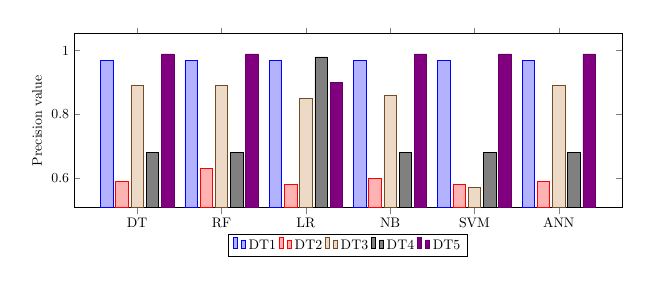
\begin{tikzpicture}[scale=0.5]
 %\centering
\begin{axis}[
     height=6cm, width=15.5cm,
    bar width=0.4cm,
    ybar,
    %ybar=5pt,% configures `bar shift'
    bar width=9pt,
    enlargelimits=0.15,
    legend style={at={(0.5,-0.15)},
    anchor=north,legend columns=-1},
    ylabel={Precision value},
    symbolic x coords={{DT,RF,LR,NB,SVM,ANN}},
    xtick=data,
    %nodes near coords,
    nodes near coords align={vertical},
    ]
\addplot coordinates {(DT,0.97) (RF, 0.97) (LR,0.97)(NB, 0.97)(SVM,0.97)(ANN, 0.97)};
\addplot coordinates{(DT,0.59) (RF, 0.63) (LR,0.58)(NB, 0.60)(SVM,0.58)(ANN, 0.59)};
\addplot coordinates {(DT,0.89) (RF, 0.89) (LR,0.85)(NB, 0.86)(SVM,0.57)(ANN, 0.89)};
\addplot coordinates {(DT,0.68) (RF, 0.68) (LR,0.98)(NB, 0.68)(SVM,0.68)(ANN, 0.68)};
\addplot coordinates {(DT,0.99) (RF, 0.99) (LR,0.90)(NB, 0.99)(SVM,0.99)(ANN, 0.99)};
\legend{DT1,DT2,DT3,DT4,DT5}
\end{axis}
\end{tikzpicture}
}
\caption{Precision values of compared classifiers on different datasets}\label{fig:precision}
\end{figure}
%
\begin{figure}[h]
\resizebox{\textwidth}{!}{
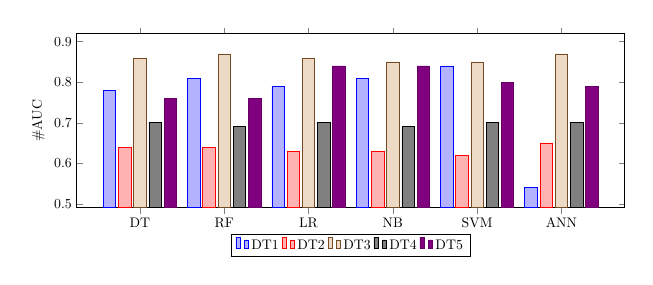
\begin{tikzpicture}[scale=0.5]
 \centering
\begin{axis}[
    height=6cm, width=15.5cm,
    bar width=0.4cm,
    ybar,
    %ybar=5pt,% configures `bar shift'
    bar width=9pt,
    enlargelimits=0.15,
    legend style={at={(0.5,-0.15)},
    anchor=north,legend columns=-1},
    ylabel={\#AUC},
    symbolic x coords={{DT,RF,LR,NB,SVM,ANN}},
    xtick=data,
    %nodes near coords,
    nodes near coords align={vertical},
    ]
\addplot coordinates {(DT,0.78) (RF, 0.81) (LR,0.79)(NB, 0.81)(SVM,0.84)(ANN, 0.54)};
\addplot coordinates{(DT,0.64) (RF, 0.64) (LR,0.63)(NB, 0.63)(SVM,0.62)(ANN, 0.65)};
\addplot coordinates {(DT,0.86) (RF, 0.87) (LR,0.86)(NB, 0.85)(SVM,0.85)(ANN, 0.87)};
\addplot coordinates {(DT,0.70) (RF, 0.69) (LR,0.70)(NB, 0.69)(SVM,0.70)(ANN, 0.70)};
\addplot coordinates {(DT,0.76) (RF, 0.76) (LR,0.84)(NB, 0.84)(SVM,0.80)(ANN, 0.79)};
\legend{DT1,DT2,DT3,DT4,DT5}
\end{axis}
\end{tikzpicture}
}
\caption{Comparison of the AUC values of the ML algorithms on different datasets}\label{fig:auc}
\end{figure}
While an one-all-fits algorithm cannot be deduced from our tests, by closely analyzing the overall performance measures one can observe that RF, LR, SVM, and ANN generally outperform the others for each dataset.  Another important result is that ML algorithms have better precision than RDT 	at least for DT1. 






% Data Preparation
\subsection{Discussion}
In this study, the algorithms DT, RF, LR, NB, SVM and ANN were applied on five datasets concerning patients with or without malaria and living in regions of Senegal namely: Diourbel, Thies and Fatick. Indeed, in order to offer a new technique for diagnosing and predicting malaria, it is important to know the performance of those existing through our datasets.
Analysing in details the performance of our six classifiers across the five datasets, the results show that there is not necessarily a single best classification algorithm, but that the best performing algorithm will depend on the characteristics of the dataset to analyze. Indeed we notice that all the algorithms produce their best precision on the DT1, DT3, and DT5 data sets. These values, which reach 97\% at times, outperform the Rapid Diagnosis Test which is the standard diagnostic tool largely adopted in the healthcare system in Senegal.
\begin{figure}
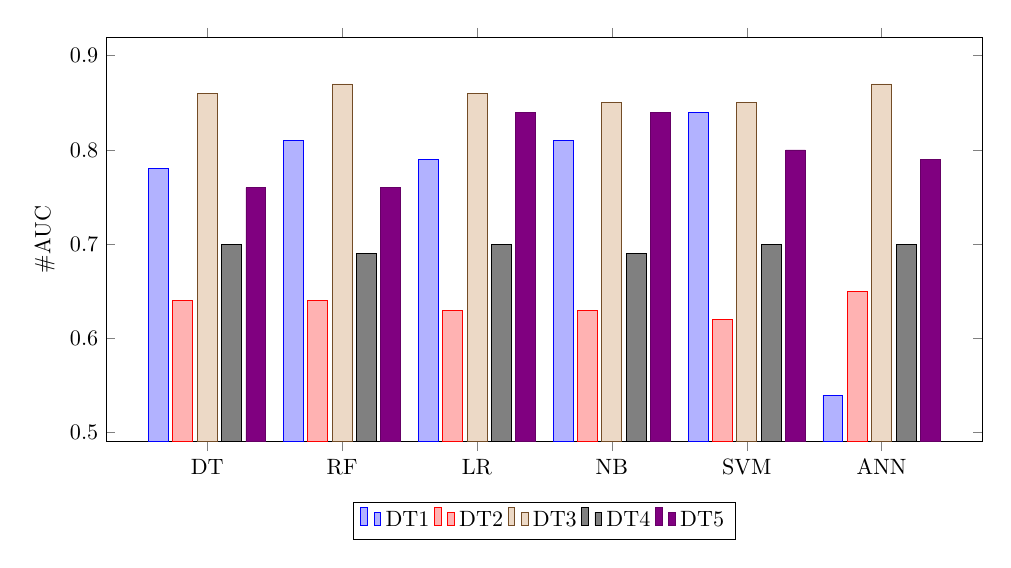
\begin{tikzpicture}[scale=0.8]
 \centering
\begin{axis}[
    height=8cm, width=15.5cm,
    bar width=0.4cm,
    ybar,
    %ybar=5pt,% configures `bar shift'
    bar width=9pt,
    enlargelimits=0.15,
    legend style={at={(0.5,-0.15)},
    anchor=north,legend columns=-1},
    ylabel={\#AUC},
    symbolic x coords={{DT,RF,LR,NB,SVM,ANN}},
    xtick=data,
    %nodes near coords,
    nodes near coords align={vertical},
    ]
\addplot coordinates {(DT,0.78) (RF, 0.81) (LR,0.79)(NB, 0.81)(SVM,0.84)(ANN, 0.54)};
\addplot coordinates{(DT,0.64) (RF, 0.64) (LR,0.63)(NB, 0.63)(SVM,0.62)(ANN, 0.65)};
\addplot coordinates {(DT,0.86) (RF, 0.87) (LR,0.86)(NB, 0.85)(SVM,0.85)(ANN, 0.87)};
\addplot coordinates {(DT,0.70) (RF, 0.69) (LR,0.70)(NB, 0.69)(SVM,0.70)(ANN, 0.70)};
\addplot coordinates {(DT,0.76) (RF, 0.76) (LR,0.84)(NB, 0.84)(SVM,0.80)(ANN, 0.79)};
\legend{DT1,DT2,DT3,DT4,DT5}
\end{axis}
\end{tikzpicture}
\caption{Comparison of the ROC Curves of the classifiers on differents datasets}
\end{figure}
However, on these same datasets, the algorithms often present very low specificities, for example 0.05 on DT1. This shows that our best performing classifiers are only able to predict a single class: either the patient has malaria or he does not, but not in both spots. This is because the DT1 and DT3 datasets are very unbalanced. In fact in these datasets either the number of patients with malaria is greater than those who are not or the opposite is true. Furthermore, we note that on the DT2 and DT4 datasets all the algorithms present specificities and Sensivity that are significant and quite similar. Contrary to what is quoted a little above, on these datasets the algorithms are efficient on the prediction tasks of the two classes. Looking closely at the results in terms of precision, recall and F-measure we observe that the classifiers RF, LR, SVM and ANN generally outperform the others for each dataset. Indeed, for the dataset DT1, which contains observations on patients living in different regions of Senegal, these four classifiers have an accuracy of 99\%, a recall greater than 92\% and an F-measure greater than 95\%. We note the same trend with the DT2 dataset which contains observations on patients living in the same area in Senegal. It can also be noted that RF, LR, SVM and ANN have better precision than the rapid diagnostic test carried out and systematically used in the majority of health structures in Senegal. This observation remains true with DT4 which is a perfectly balanced dataset. In conclusion, it is very difficult or even impossible for us to say definitively which algorithm is more efficient for the task of predicting malaria, but the choice of this one will strongly depend on the choice of the data set. However, this study shows that our classification problem has been taken care of. A method integrating several models and various datasets is necessary

\begin{figure}
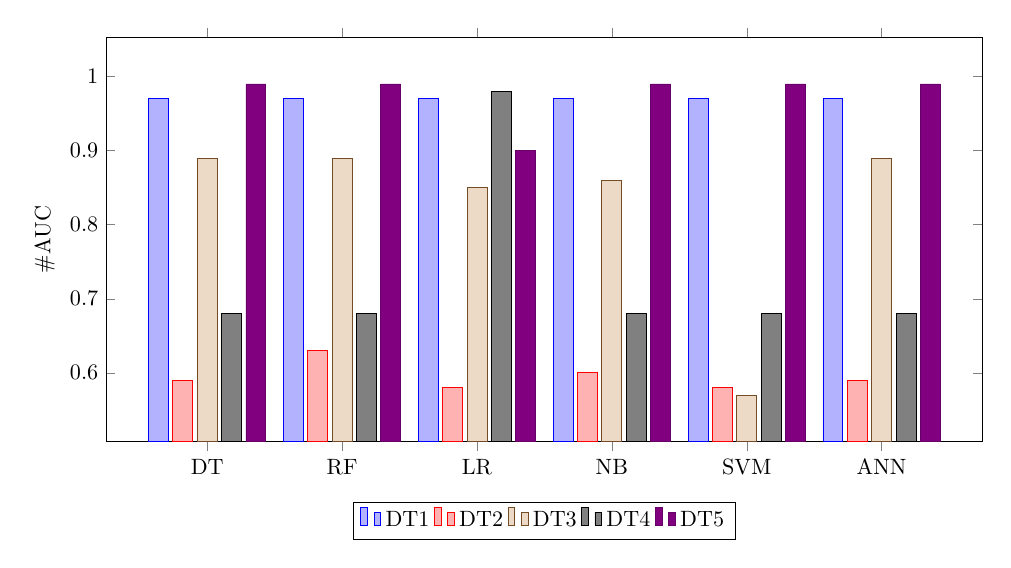
\begin{tikzpicture}[scale=0.8]
 \centering
\begin{axis}[
    height=8cm, width=15.5cm,
    bar width=0.4cm,
    ybar,
    %ybar=5pt,% configures `bar shift'
    bar width=9pt,
    enlargelimits=0.15,
    legend style={at={(0.5,-0.15)},
    anchor=north,legend columns=-1},
    ylabel={\#AUC},
    symbolic x coords={{DT,RF,LR,NB,SVM,ANN}},
    xtick=data,
    %nodes near coords,
    nodes near coords align={vertical},
    ]
\addplot coordinates {(DT,0.97) (RF, 0.97) (LR,0.97)(NB, 0.97)(SVM,0.97)(ANN, 0.97)};
\addplot coordinates{(DT,0.59) (RF, 0.63) (LR,0.58)(NB, 0.60)(SVM,0.58)(ANN, 0.59)};
\addplot coordinates {(DT,0.89) (RF, 0.89) (LR,0.85)(NB, 0.86)(SVM,0.57)(ANN, 0.89)};
\addplot coordinates {(DT,0.68) (RF, 0.68) (LR,0.98)(NB, 0.68)(SVM,0.68)(ANN, 0.68)};
\addplot coordinates {(DT,0.99) (RF, 0.99) (LR,0.90)(NB, 0.99)(SVM,0.99)(ANN, 0.99)};
\legend{DT1,DT2,DT3,DT4,DT5}
\end{axis}
\end{tikzpicture}
\caption{Precision values of compared classifiers on different datasets}

\end{figure}


\begin{figure}
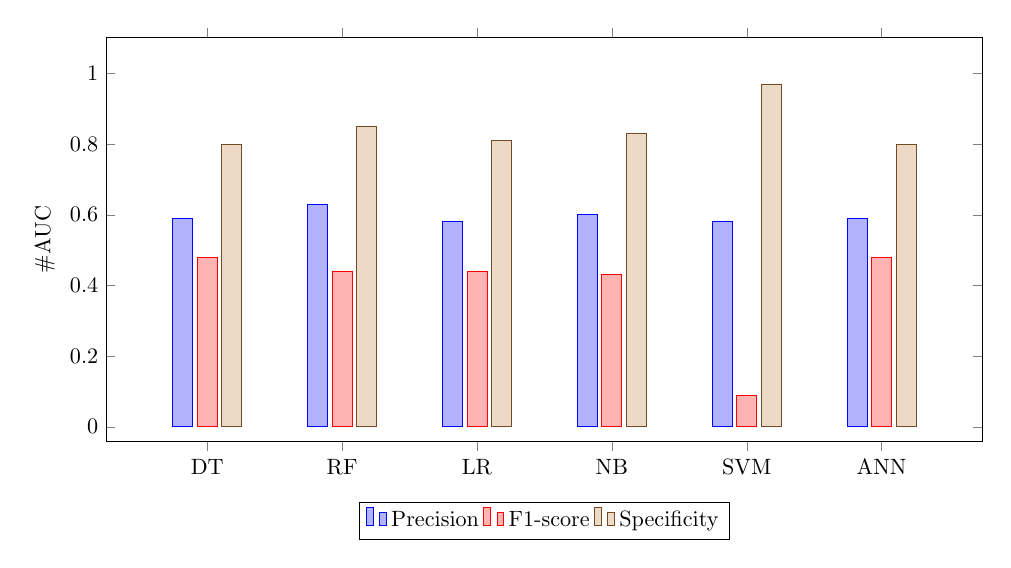
\begin{tikzpicture}[scale=0.8]
 \centering
\begin{axis}[
    height=8cm, width=15.5cm,
    bar width=0.4cm,
    ybar,
    %ybar=5pt,% configures `bar shift'
    bar width=9pt,
    enlargelimits=0.15,
    legend style={at={(0.5,-0.15)},
    anchor=north,legend columns=-1},
    ylabel={\#AUC},
    symbolic x coords={{DT,RF,LR,NB,SVM,ANN}},
    xtick=data,
    %nodes near coords,
    nodes near coords align={vertical},
    ]
\addplot coordinates {(DT,0.59) (RF, 0.63) (LR,0.58)(NB, 0.60)(SVM,0.58)(ANN, 0.59)};
\addplot coordinates{(DT,0.48) (RF, 0.44) (LR,0.44)(NB, 0.43)(SVM,0.09)(ANN, 0.48)};
\addplot coordinates {(DT,0.80) (RF, 0.85) (LR,0.81)(NB, 0.83)(SVM,0.97)(ANN, 0.80)};
%\addplot coordinates {(DT,0.68) (RF, 0.68) (LR,0.98)(NB, 0.68)(SVM,0.68)(ANN, 0.68)};
%\addplot coordinates {(DT,0.99) (RF, 0.99) (LR,0.90)(NB, 0.99)(SVM,0.99)(ANN, 0.99)};
\legend{Precision,F1-score,Specificity,DT4}
\end{axis}
\end{tikzpicture}
\caption{Precison, F1-score, specificity values of the classifiers on DT1}

\end{figure}
\section{Conclusion}
In this study, six classifiers using a wide variety of operating procedures have been extensively tested and compared over real world health datasets in order to evaluate their performance for the task of predicting the occurrence or not of Malaria in a patient knowing his signs and symptoms. The results obtained show that the algorithms RF, LR,
SVM with Gaussian kernel and ANN present the best performances in predicting the occurrence or not of Malaria. In addition those four algorithms outperform the Rapid Diagnosis Test which is the standard diagnostic tool largely adopted in the health system in
Senegal. This research has indicated that in practice there is no single best classification tool, but instead the best technique will on the characteristics of the dataset to be analysed. 
Future work consists in the study and the implementation of an ensemble method for predicting the occurrence or not of malaria based on the classifiers offering the best performances in our present study. But also to compare these performances with the ensemble methods for their validation





\bibliographystyle{vancouver}
\bibliography{../biblio}
\end{document}
